\subsection{Noise Generation}\paragraph{}
To actually achieve the wispy shape of a cloud we use an existing soft-particle noise implementation. 

For this implementation we first generate a semi-transparent noise volume using gradient densities. The final result is a signed 3D texture with randomly generated RGB and variable alpha values.

% noise texture
\begin{figure}[h]
\centering
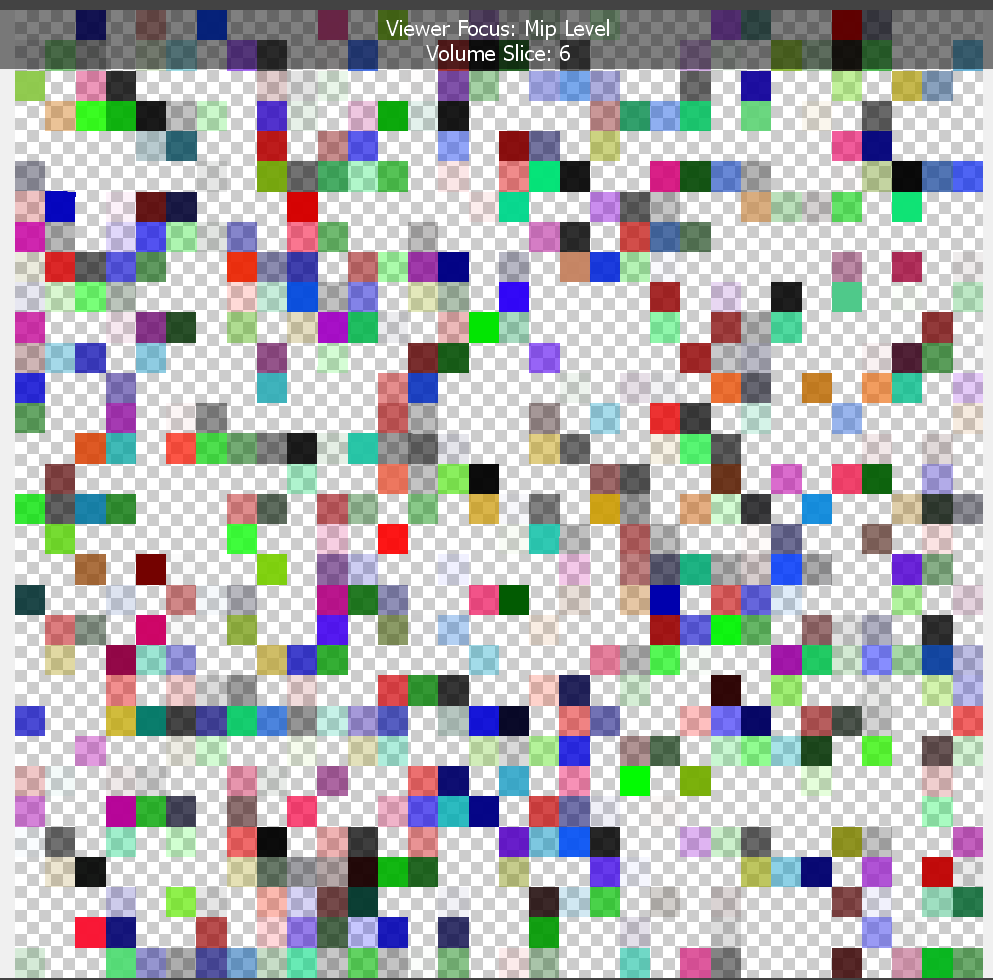
\includegraphics[width=0.7\textwidth]{../res/noiseslice.png}
\caption{1 of 32 slices in the noise texture}
\end{figure}

To represent this noise texture, we follow a similar process as our first pass voxelization: for every billboard we calculate a spherical distribution. Using this distribution we find the near and far positions on the sphere respective to the current fragment. We start at the near position and iterate through the sphere to the back. On each step, we sample the noise texture across several octaves. 

When sampling the noise texture, we add an offset that updates with run-time. This causes our sampling coordinates to translate through the noise volume over time creating an animating effect. The final result is convincing fog.

% gray fog
\begin{figure}[h]
\centering
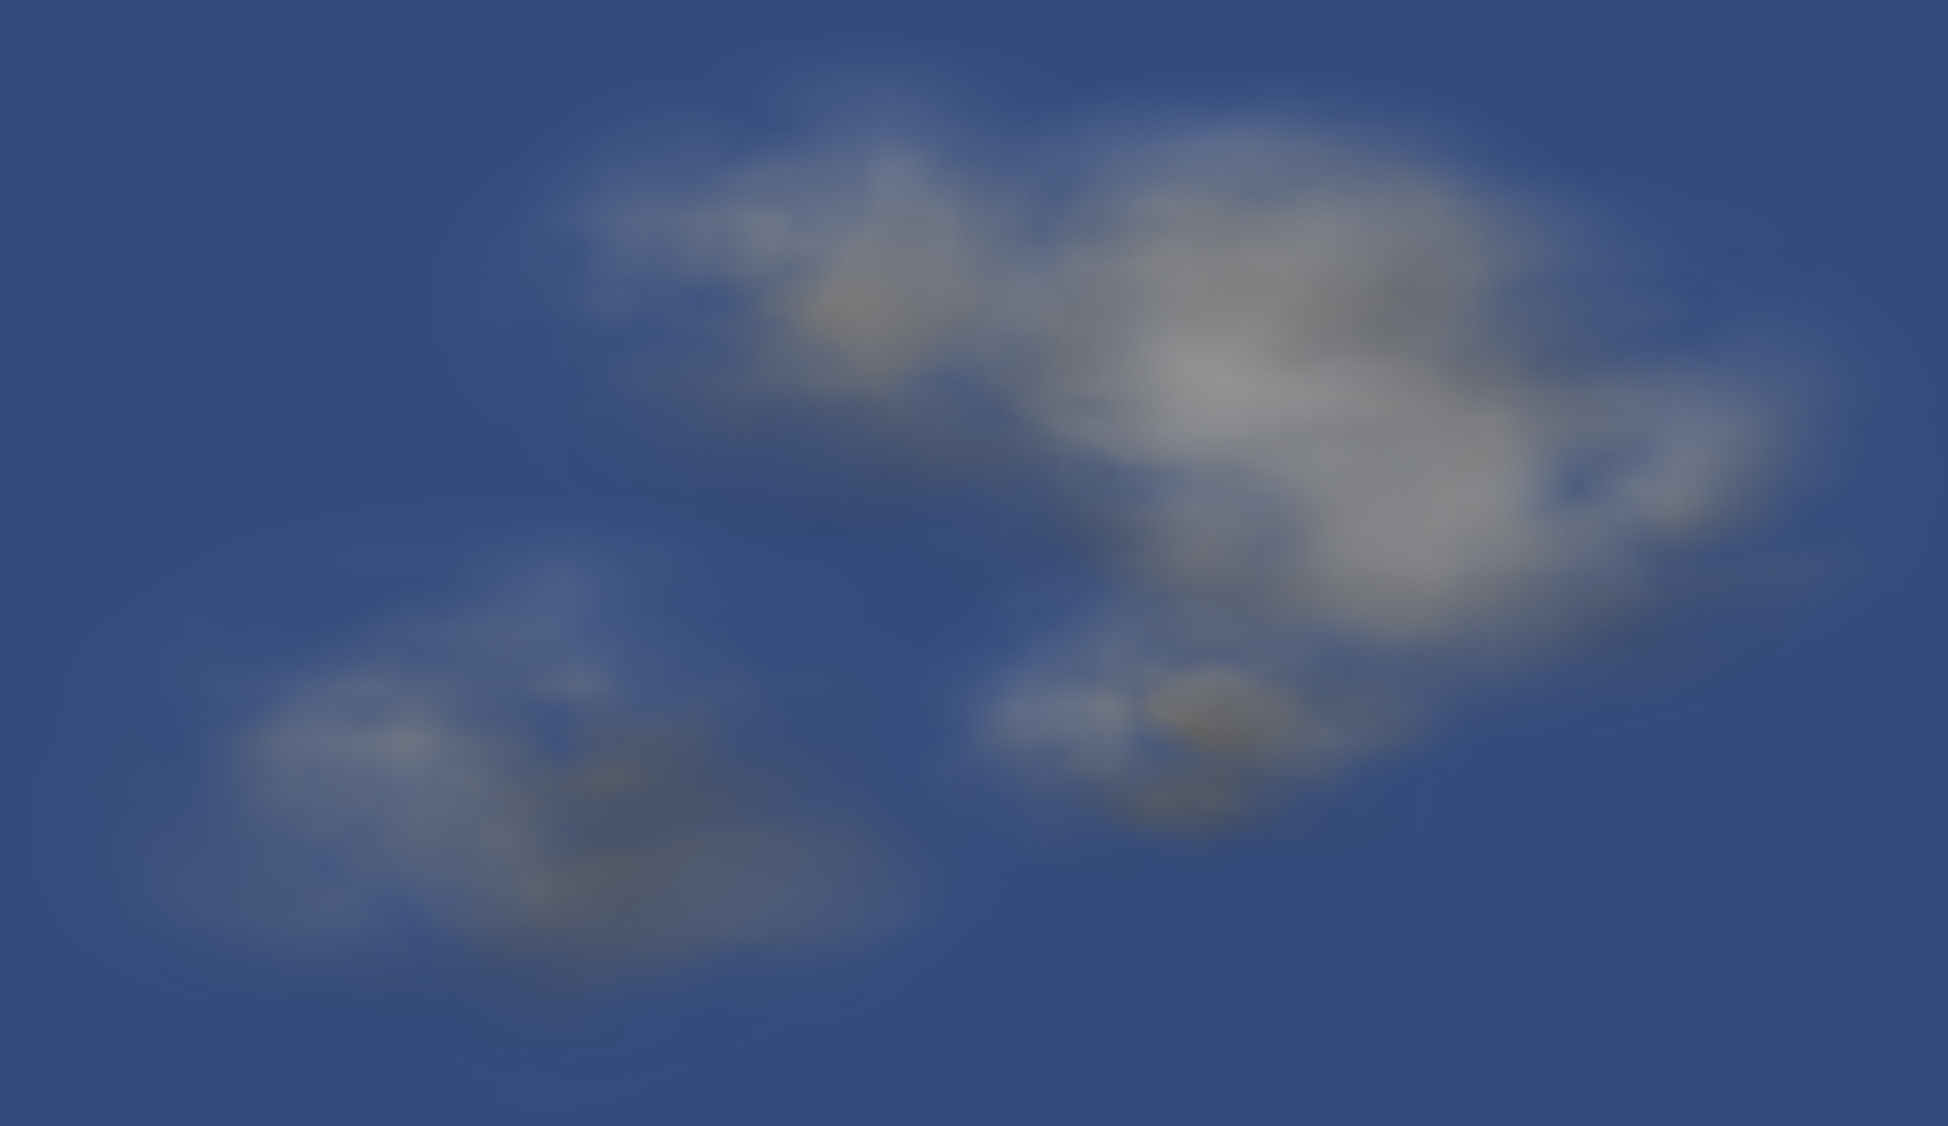
\includegraphics[width=\textwidth]{../res/fog.png}
\caption{Noise-based fog using 10 billboards}
\end{figure}


